\documentclass{beamer}
\usepackage[utf8]{inputenc}
\usepackage[T1]{fontenc}
\usepackage{courier}
\usepackage{etoolbox}

\usepackage{tabularx} % package that allows dynamical changing table cell width
\usepackage{multirow}  % package that enables multiple rows in a table

\usepackage{amsfonts}
\usepackage{booktabs}
\usetheme{Rochester}

\definecolor{chameleongreen1}{RGB}{98,189,25}
\definecolor{chameleongreen2}{RGB}{188,225,141}
\definecolor{chameleongreen3}{RGB}{51,149,48}
\definecolor{chameleongreen4}{RGB}{0,98,90}

\definecolor{darkyellow}{RGB}{204,204,0}

\setbeamercolor*{palette primary}{fg=white,bg=chameleongreen2}
\setbeamercolor*{palette secondary}{fg=white,bg=chameleongreen3}
\setbeamercolor*{palette tertiary}{fg=white,bg=chameleongreen4}
\setbeamercolor*{palette quaternary}{fg=white,bg=chameleongreen1}

\setbeamercolor*{titlelike}{bg=chameleongreen1}
\setbeamercolor*{frametitle}{bg=chameleongreen1,fg=black}
\setbeamercolor*{part title}{bg=chameleongreen1,fg=black}
\setbeamercolor*{item}{fg=chameleongreen1}

% \newcommand{\ComArg}{\mbox{\textsc{ComArg}}\xspace}

\setbeamercolor{block}{fg=chameleongreen1}
\setbeamercolor{block title}{bg=chameleongreen1,fg=black}

\newcommand{\pro}[1]{\textcolor{green}{#1}}
\newcommand{\con}[1]{\textcolor{red}{#1}}
% Colors.
\setbeamercolor*{lineup}{parent=palette primary}
\setbeamercolor*{linemid}{parent=palette secondary}
\setbeamercolor*{linebottom}{parent=palette tertiary}
\setbeamercolor*{title page header}{parent=palette quaternary}

\AtBeginSection[]
{
\begin{frame}
\frametitle{Overview}
\tableofcontents[currentsection,currentsubsection]
\end{frame}
}

\AtBeginSubsection[]
{
  \begin{frame}%<beamer>
    \frametitle{Overview}
    \tableofcontents[
        currentsection,
        currentsubsection,
	subsectionstyle=show/shaded
    ]
  \end{frame}
}

\setbeamerfont{page number in head/foot}{size=\large}
\setbeamertemplate{footline}[frame number]

\scriptsize{ \bibliographystyle{apalike}}

\title{
	Computational Methods for \\
	Argumentation Mining of Claims \\
	in Internet Discussions
}
\author{student: mag.~ing.~comp.~Filip Boltužić 
\\ mentor: izv.~prof.~dr.~sc.~Jan Šnajder
}
\institute{
Faculty of Electrical Engineering and Computing \\
University of Zagreb
}

\titlegraphic{
\includegraphics[width=0.3\textwidth,height=0.15\textheight]{logoi.jpg}}

\date{September 29th, 2020}

\begin{document}

%%%%%%%%%%%%%%%%%%%%%%%%%%%%%%%%%%%%%%%%%%%%%%%%%%%%%%%%%%%%%%%%
{
\setbeamertemplate{footline}{}
\begin{frame}
\titlepage
\end{frame}
}

\setcounter{framenumber}{0}

%%%%%%%%%%%%%%%%%%%%%%%%%%%%%%%%%%%%%%%%%%%%%%%%%%%%%%%%%%%%%%%%

\begin{frame}
\frametitle{Should masks be worn to prevent virus spreading?}
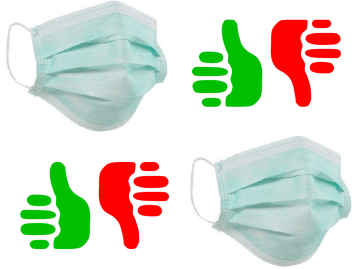
\includegraphics[scale=0.3]{MaskProCon.png}
\footnote{
\tiny{Source: \url{https://www.medwiser.org/pros-cons-of-public-recommendations-for-surgical-cloth-diy-masks-to-prevent-coronavirus/}}}
\end{frame}

\begin{frame}
\frametitle{Should masks be worn to prevent virus spreading?}
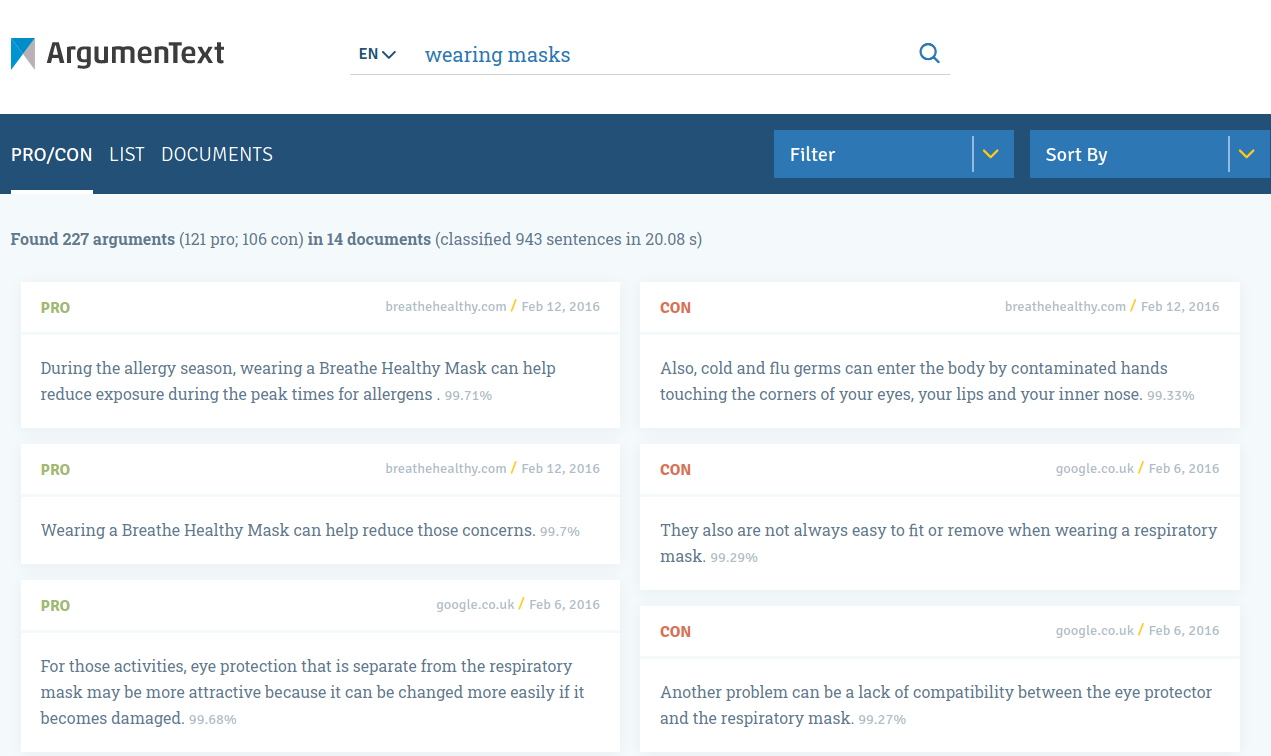
\includegraphics[width=\textwidth,height=0.9\textheight]{argument_text.png}
\footnote{
\tiny{Source: \url{http://argumentsearch.com/search/?query=wearingmasks&language=en}}}
\end{frame}

\begin{frame}
\frametitle{Should masks be worn to prevent virus spreading?}
\begin{block}{Pro Claims}
\begin{itemize}
	\item Wearing a Breathe Healthy Mask can help reduce the amount of particles you breathe.
	\item Wearing a facemask properly offers satisfactory protection against respiratory tract infections.
\end{itemize}
\end{block}

\begin{block}{Con Claims}
\begin{itemize}
	\item Also, cold and flu germs can enter the body by contaminated hands touching the corners of your eyes, your lips and your inner nose.
	\item During the allergy season, wearing a Breathe Healthy Mask can help reduce exposure during the peak times for allergens
\end{itemize}
\end{block}

\end{frame}

%%%%%%%%%%%%%%%%%%%%%%%%%%%%%%%%%%%%%%%%%%%%%%%%%%%%%%%%%%%%%%%%
\begin{frame}
\frametitle{How to automate argument extraction from text?}
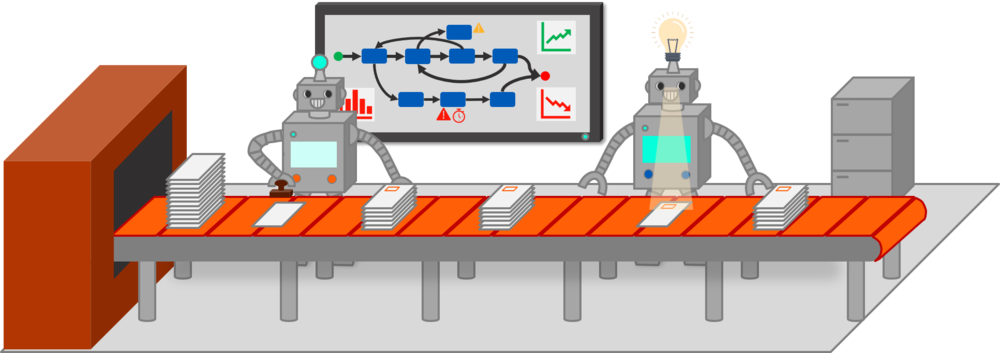
\includegraphics[scale=0.3]{assembly_line.png}
\footnote{
\tiny{Source: \url{https://www.finbridge.de/trends/2019/7/9/how-to-rpa}}}
\end{frame}
%%%%%%%%%%%%%%%%%%%%%%%%%%%%%%%%%%%%%%%%%%%%%%%%%%%%%%%%%%%%%%%%

\section{Introduction}

%%%%%%%%%%%%%%%%%%%%%%%%%%%%%%%%%%%%%%%%%%%%%%%%%%%
%=================================================%
%%%%%%%%%%%%%%%%%%%%%%%%%%%%%%%%%%%%%%%%%%%%%%%%%%%

\begin{frame}
	\frametitle{Argumentation}

\begin{block}{Argumentation}
Argumentation is the process of putting forth arguments to determine  the
acceptability of claims \cite{walton1989informal}.
\end{block}

\begin{block}{Argument}
An argument links a set of claims, the premises, to another claim, the conclusion
\cite{walton1989informal}.
\end{block}
\end{frame}

%%%%%%%%%%%%%%%%%%%%%%%%%%%%%%%%%%%%%%%%%%%%%%%%%%%
%=================================================%
%%%%%%%%%%%%%%%%%%%%%%%%%%%%%%%%%%%%%%%%%%%%%%%%%%%

\begin{frame}

\frametitle{Argumentation Mining}
\begin{block}{Argumentation Mining}
Argumentation mining is a discipline dealing with the automatic identification and extraction
of the structure of inference and reasoning expressed as arguments presented in natural language
\cite{lawrence2019argument}.
\end{block}

\vspace{1cm}
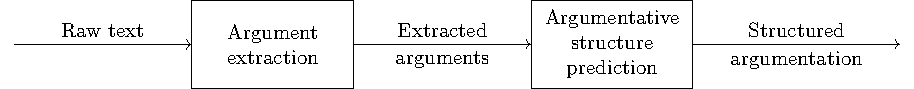
\includegraphics[scale=0.7]{../area_description_pipeline-figure0.pdf}
\end{frame}

%%%%%%%%%%%%%%%%%%%%%%%%%%%%%%%%%%%%%%%%%%%%%%%%%%%
%=================================================%
%%%%%%%%%%%%%%%%%%%%%%%%%%%%%%%%%%%%%%%%%%%%%%%%%%%

\begin{frame}
\frametitle{Argumentation Mining Application}

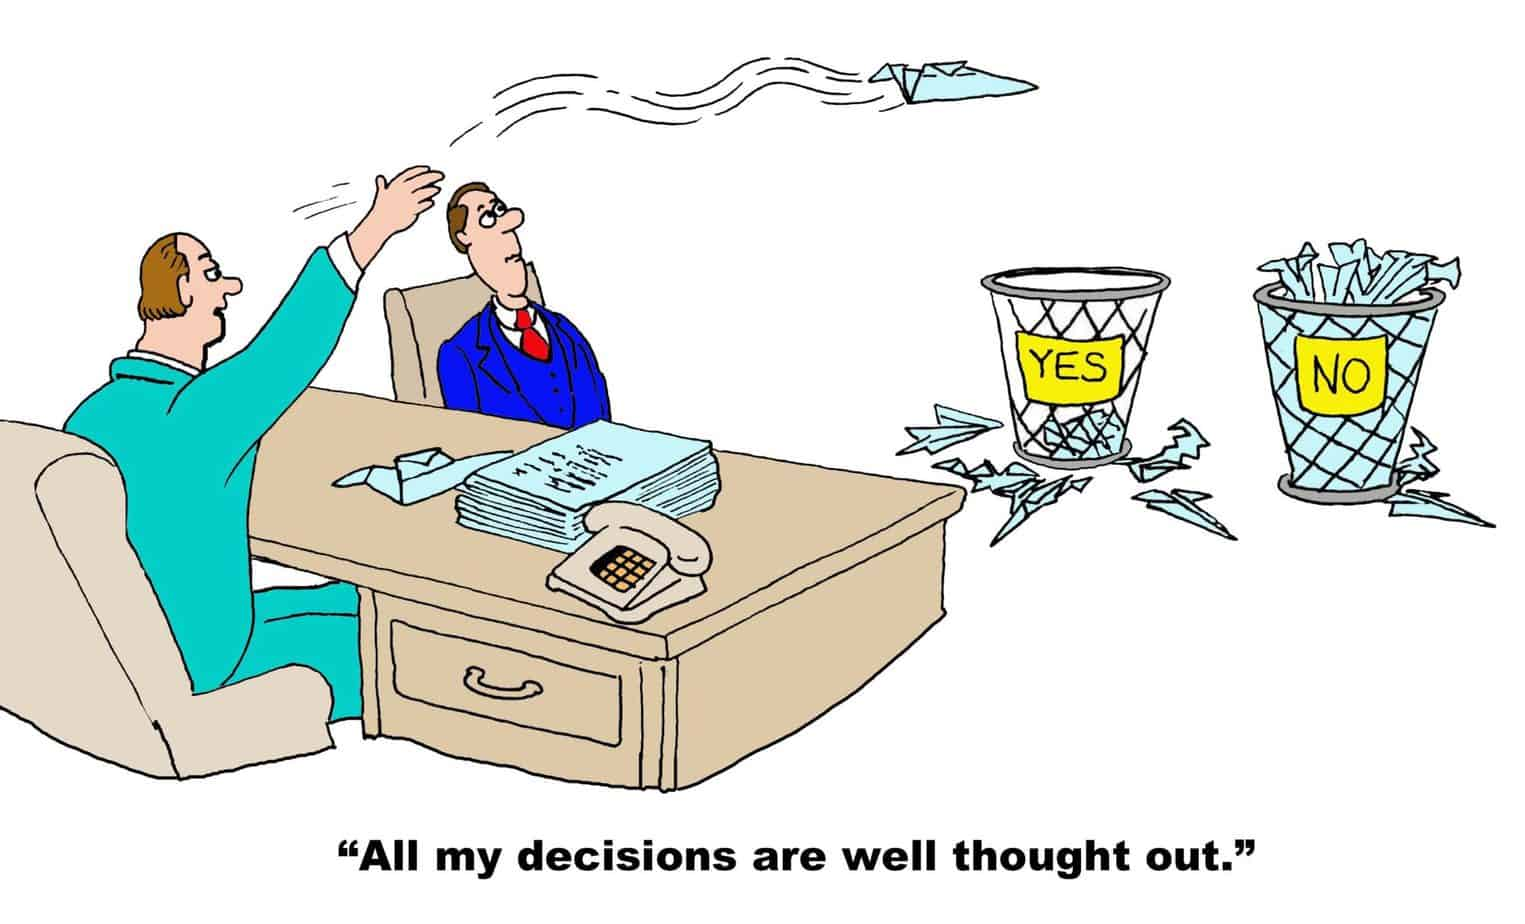
\includegraphics[scale=0.2]{informed_decision.jpeg}
\footnote{
\tiny{Source: \url{https://hadit.com/an-insulting-promotion-at-veterans-affairs/}}}

\end{frame}

\begin{frame}
\frametitle{Argumentation Mining Related Areas}

\begin{itemize}
\item Stance Classification
	\begin{itemize}
		\item Determines \textcolor{green}{Pro} or \textcolor{red}{Con} stance of claim towards a topic
	\end{itemize}
\item Fact Checking
	\begin{itemize}
		\item Checks factual assertions in non-fictional text to determine the
			veracity and correctness of the factual statements
	\end{itemize}
\item Sentiment Classification
	\begin{itemize}
		\item Determines subjective information and affective states in text
	\end{itemize}
\item Rumour Tracking
	\begin{itemize}
		\item Objective is to find the source of rumourous claims
	\end{itemize}
\end{itemize}

\end{frame}

\begin{frame}
\frametitle{Argumentation Mining Approaches}

\begin{itemize}
\item Unstructured Argumentation Mining
	\begin{itemize}
		\item Employs methods unaware of argument structure
		\item Usually attempts to derive arguments directly from text
		\item Offer little to none interpretability
		\item Do not require a background knowledge
	\end{itemize}
\item Structured Argumentation Mining
	\begin{itemize}
		\item Involves biased methods on what arguments are and typically consist of
		\item Produces a formal logical structure of arguments
		\item Requires background knowledge
	\end{itemize}
\end{itemize}

\end{frame}

%%%%%%%%%%%%%%%%%%%%%%%%%%%%%%%%%%%%%%%%%%%%%%%%%%%
%=================================================%
%%%%%%%%%%%%%%%%%%%%%%%%%%%%%%%%%%%%%%%%%%%%%%%%%%%

\section{Unstructured Argumentation Mining of Claims}

\subsection{Claim Clustering}

\begin{frame}
	\frametitle{Claim Clustering}
	\begin{block}{Goal}
		Find the most prominent claims from a discussion
	\end{block}

	\begin{block}{Approach}
		Cluster claims and use centroids of clusters as prominent claims
	\end{block}
\end{frame}

%%%%%%%%%%%%%%%%%%%%%%%%%%%%%%%%%%%%%%%%%%%%%%%%%%%
%=================================================%
%%%%%%%%%%%%%%%%%%%%%%%%%%%%%%%%%%%%%%%%%%%%%%%%%%%

\begin{frame}
	\frametitle{Claim Clustering -- Data}
	\begin{itemize}
		\item Dataset of user posts annotated with prominent claims \cite{hasan2014you}
		\item Four debate topics: 
		``Obama'', ``Marijuana'', ``Gay rights'', and ``Abortion'' 
	\item 3104 claims (``Abortion'' 814, ``Gay rights'' 824, ``Marijuana'' 836, and ``Obama'' 630) and 
		47 different prominent claims (25 \textcolor{green}{pro} and 22 \textcolor{red}{con})
	\end{itemize}
\end{frame}

%%%%%%%%%%%%%%%%%%%%%%%%%%%%%%%%%%%%%%%%%%%%%%%%%%%
%=================================================%
%%%%%%%%%%%%%%%%%%%%%%%%%%%%%%%%%%%%%%%%%%%%%%%%%%%

\begin{frame}
	\frametitle{Claim Clustering -- Model}
	Similarity
\begin{enumerate} 
\item a bag-of-word (BoW) vector, weighted
by inverse sentence frequency \cite{ramage2009random} and 
\item a distributed representation based on the skip-gram model
	\cite{mikolov2013distributed}. 
\end{enumerate}
\vspace{0.5cm}
Clustering Algorithm
\begin{itemize}
	\item hierarchical agglomerative clustering (HAC) algorithm \cite{szekely2005hierarchical}
	\item linkage between clusters $A$ and $B$
		\begin{itemize}
			\item Complete: $\max \{d(a, b): a \in A, b \in B\}$
			\item Ward's:
		$$
		\sum_{i \in A \cup B} ||x_i - m_{A \cup B}||^2 - \sum_{i \in A}||x_i - m_A||^2 
		- \sum_{i \in B} ||x_i - m_B||^2
		$$ 
		where $m_j$ is the center of cluster $j$  and $x_i$ is a datapoint
		in cluster $i$ \cite{ward1963hierarchical}.
		\end{itemize}
\end{itemize}
\end{frame}

%%%%%%%%%%%%%%%%%%%%%%%%%%%%%%%%%%%%%%%%%%%%%%%%%%%
%=================================================%
%%%%%%%%%%%%%%%%%%%%%%%%%%%%%%%%%%%%%%%%%%%%%%%%%%%

\begin{frame}
	\frametitle{Claim Clustering -- Results}

\begin{table}[t]
\begin{center}
{\tiny
\setlength{\tabcolsep}{0.5em}
\begin{tabular}{@{}l cccc cccc cccc cccc@{}}
\toprule
& \multicolumn{4}{c}{``Obama''} & \multicolumn{4}{c}{``Marijuana''} &
	\multicolumn{4}{c}{``Gay rights''} & \multicolumn{4}{c}{``Abortion''}
	\\
\cmidrule(lr){2-5}
\cmidrule(lr){6-9}
\cmidrule(lr){10-13}
\cmidrule(lr){14-17}
Model (linkage) &
$h$ & $c$ & $V$ & ARI &
$h$ & $c$ & $V$ & ARI &
$h$ & $c$ & $V$ & ARI &
$h$ & $c$ & $V$ & ARI \\
\midrule
BoW (Complete) &
.15 & .15 & .15 & .03 & 
.04 & .04 & .04 & .00 & 
.04 & .04 & .04 & .01 & 
.05 & .04 & .04 & .01\\
%.153 & .150 & .152 & .025 & 
%.040 & .036 & .038 & .002 & 
%.039 & .036 & .038 & .007 & 
%.045 & .041 & .043 & .005\\
BoW (Ward's) & 
.22 & \textbf{.34} & .27 & .04 & 
.15 & .20 & .17 & .02 & 
.13 & \textbf{.17} & \textbf{.15} & .04 & 
.22 & \textbf{.27} & \textbf{.24} & .07 \\
%.218 & .342 & .266 & .042 & 
%.145 & .197 & .167 & .016 & 
%.127 & .169 & .145 & .038 & 
%.223 & .266 & .243 & .072 \\
Skip-gram (Complete) & 
.18 & .26 & .21 & .04 & 
.09 & .22 & .13 & .02 & 
.09 & .10 & .10 & .04 & 
.17 & .24 & .20 & .03  \\
%.177 & .261 & .211 & .041 & 
%.094 & .216 & .131 & .021 & 
%.089 & .104 & .096 & .043 & 
%.167 & .242 & .198 & .026  \\
Skip-gram (Ward's) & 
\textbf{.30} & .29 & \textbf{.30} & \textbf{.10} & 
\textbf{.25} & \textbf{.24} & \textbf{.25} & \textbf{.19} & 
\textbf{.16} & .15 & \textbf{.15} & \textbf{.07} & 
\textbf{.24} & .22 & .23 & \textbf{.08} \\
%.300 & .294 & .297 & .102 & 
%.250 & .242 & .246 & .186 & 
%.156 & .152 & .154 & .072 & 
%.235 & .217 & .226 & .078 \\
 \\
\bottomrule
\end{tabular}}
\caption{External evaluation of clustering models on the four topics using 
	homogeneity ($h$), completeness ($c$), V-measure ($V$), and adjusted
	Rand index (ARI) }
\label{tab:external-eval}
\end{center}
\end{table}

\end{frame}

%%%%%%%%%%%%%%%%%%%%%%%%%%%%%%%%%%%%%%%%%%%%%%%%%%%
%=================================================%
%%%%%%%%%%%%%%%%%%%%%%%%%%%%%%%%%%%%%%%%%%%%%%%%%%%

\begin{frame}
	\frametitle{Claim Clustering -- Results}

\begin{table}[ht]
\setlength{\tabcolsep}{0.4em}
{\tiny
\begin{center}
\begin{tabular}{lp{1cm}p{3cm}|lp{1cm}p{3cm}}
\toprule
\multicolumn{3}{c}{Hypothesized clustering} & \multicolumn{3}{c}{Gold classes}\\
\cmidrule(lr){1-3}\cmidrule(lr){4-6}
Id & Classes & Cluster medoid & Id & Clusters & Gold prominent claim \\
\midrule
%1 &  \textbf{10 (54\%)}  \newline  2 (12\%)  \newline  6 (10\%)  &

%\emph{%
%Tobacco and alcohol are both legal and widely used in the US, (...) If the abuse of marijuana is harmful, isn't the abuse of tobacco or alcohol equally life threatening? (...)
%} &
%
%1  &  5 (23\%) \newline 9 (19\%) \newline 10 (18\%) 
% &
% \emph{Prohibition violates human rights}
\\
% \midrule
2 & \textbf{4 (92\%) } \newline  9 (8\%) &
\emph{The biggest effect would be an end to brutal mandatory sentencing of long
	jail times that has ruined so many young peoples lives.
}
& 
4  &  9 (40\%) \newline 3 (26\%) \newline 10 (12\%)  
&
\emph{%
%it is not the governments place to control personal aspects of my life that would have no affect on anyone else.
Prohibition violates human rights
}
\\
\midrule

8 &  \textbf{9 (92\%)} &
\emph{%
the economy would get billions of dollars in a new industry if it were
legalized (...) no longer would this revenue go directly into the black market.
} 
& 
9 &  8 (53\%) \newline 3 (25\%) \newline 9 (10\%) 
&
\emph{%
%Not only would it be better for the economy, but look at Amsterdam - weed is legal over there and you never hear anything out of them. They've been onto something for a long time now.
Legalized marijuana can be controlled and regulated by the government
}
% \str{%
% The biggest effect would be an end to brutal mandatory sentencing of long jail times that has ruined so many young peoples lives.
% } 
% & 
% 2  &  1 (33\%) \newline 9 (28\%) \newline 3 (15\%) 
% &
% \str{%
% %(...) I think it ridiculous that people want to legalise something that has four - seven times the amount of tar (the cancer causing agent) in one cone than in one cigarette (...)
% Responsible for brain damage
% }
% 
% \\
% \midrule
% 3 &  \textbf{9 (44\%)}  \newline  4 (25\%)  \newline 7 (8\%) &
% \str{%
% Legalizing pot alone would not end the war on drugs. It would help (...) my personal opinion would be the only way to completely end the war on drugs would be to legalize everything. 
% } 
% & 3  &  9 (41\%) \newline 3 (23\%) \newline 10 (23\%) 
% &
% \str{%
% %Worst case scenario, half the population would go out and buy it, get high and wreak havoc on America. Productivity would go down :) and some people would simply do reckless things.
% Causes crime
% }
% 
% \\
% \midrule
% 4 &  \textbf{8 (37\%)}  \newline  1 (22\%)  \newline  10 (17\%)   & 
% \str{%
% What all these effects have in common is that they result from changes in the brain's control centers (...) So, when marijuana disturbs functions centered in the deep control centers, disorienting changes in the mind occur (...)
% } &
% 4  &  9 (40\%) \newline 3 (26\%) \newline 10 (12\%)  
% &
% \str{%
% %it is not the governments place to control personal aspects of my life that would have no affect on anyone else.
% Prohibition violates human rights
% }
% \\
% \midrule
% 5 &  \textbf{1 (45\%)}  \newline  6 (18\%)  \newline  8 (10\%)  & 
% \str{%
% People with pre-existing mental disorders also tend to abuse alcohol and tobacco. (...) the link between marijuana use and mental illness may be an instance when correlation does not equal causation. 
% } 
% &
% 5  &  6 (25\%) \newline 7 (25\%) \newline 4 (18\%) 
% &
% \str{%
% %you also have to consider that continuous usage of LSD can cause severe mental illnesses in people. There hasn't ever been a case of this happening from using marijuana.
% Does not cause any damage to our bodies
% }
% \\
% \midrule
% 6 &  \textbf{5 (63\%)}  \newline  10 (31\%)  \newline  1 (6\%) & 
% \str{%
% There are thousands of deaths every year from tobacco and alcohol, yet there has never been a recorded death due to marijuana.
% } &
% 6  &  9 (29\%) \newline 1 (19\%) \newline 7 (16\%) 
% &
% \str{%
% %There have been many deaths directly linked to marijuana use. Car crashes are a common way in which people under the influence of marijuana harm themselves, and others.
% Damages our bodies
% }
% \\
% \midrule
% 7 &  \textbf{10 (48\%)}  \newline  5 (13\%)  \newline  6 (12\%)    &
% \str{%
% as far as it goes for medicinal purposes, marijuana does not cure anything (...) It is for the sole purpose of numbing the pain in cancer patients (...) and also making patients hungry so they eat more and gain weight on their sick bodies 
% } &
% 7  &  9 (39\%) \newline 3 (30\%) \newline 1 (9\%) 
% &
% \str{%
% %The last thing we need is more people doing it. More people making it a problem for themselves, more people ending up in rehab at the governments expense.
% Highly addictive
% }
% \\
% \midrule
% 8 &  \textbf{9 (92\%)} &
% \str{%
% the economy would get billions of dollars in a new industry if it were legalized (...) no longer would this revenue go directly into the black market.
% } 
% &
% 8  &  4 (44\%) \newline 7 (16\%) \newline 9 (16\%) 
% &
% \str{%
% %If we legalize something that makes people stop caring about their lives and only want to get "high" then we are pretty much setting a course for our downfall as a civilization.
% If legalized, people will use marijuana and other drugs more
% }
% \\
% \midrule
% 9 &  \textbf{4 (30\%)}  \newline  9 (13\%)  \newline  10 (11\%)   &
% \str{%
% (...) I think it ridiculous that people want to legalise something that has four - seven times the amount of tar (the cancer causing agent) in one cone than in one cigarette (...)
% } &
% 9  &  8 (53\%) \newline 3 (25\%) \newline 9 (10\%) 
% &
% \str{%
% %Not only would it be better for the economy, but look at Amsterdam - weed is legal over there and you never hear anything out of them. They've been onto something for a long time now.
% Legalized marijuana can be controlled and regulated by the government
% }
% \\
% \midrule
% 10 &  \textbf{10 (30\%)}  \newline  9 (19\%)  \newline  4 (15\%)   &
% \str{%
% But I'm not gonna tell anyone they can't smoke pot or do meth because I don't like it.
% } &
% 10  &  1 (36\%) \newline 7 (21\%) \newline 10 (18\%) 
% & 
% \str{%
% %I don't personally use it, or have any real want to, but I don't think it's any worse than alcohol or cigarettes.
% Not addictive
% }
 \\
\bottomrule
\end{tabular}
\caption{Manual cluster-class matching for the ``Marijuana'' topic and the gold
number of clusters. More details in \cite{boltuzic2015identifying}}
\label{tab:cluster-class}
\end{center}}
\end{table}
\end{frame}

%%%%%%%%%%%%%%%%%%%%%%%%%%%%%%%%%%%%%%%%%%%%%%%%%%%
%=================================================%
%%%%%%%%%%%%%%%%%%%%%%%%%%%%%%%%%%%%%%%%%%%%%%%%%%%

\subsection{Prominent Claim Identification}

\begin{frame}
\frametitle{Prominent Claim Identification}
	\begin{block}{Prominent Claim Identification}
The task of identifying what prominent claims, from a predefined set of
prominent claims, have been used in users' comments, and how \cite{boltuzic2014back}. 
\\
\vspace{0.5cm}

The prominent claims can be \textcolor{red}{attacked}, 
\textcolor{green}{supported} or neutral with respect to the comment.
	\end{block}
\end{frame}

\begin{frame}
\frametitle{Prominent Claim Identification -- Data}

ComArg corpus \footnote{Freely available under the CC BY-SA-NC license from
\url{http://takelab.fer.hr/data/comarg}}

\begin{itemize}
	\item prominent claims from debate platform \textit{idebate.org}
	\item comments from \textit{procon.org}
	\item two topics: ``\textit{Under God in Pledge}'' (UGIP) and 
``\textit{Gay marriage}'' (GM)
	\item 175
comments and 6 arguments for UGIP, and 198 comments and 7 arguments for GM
\end{itemize}

\end{frame}

\begin{frame}
\frametitle{Prominent Claim Identification -- Data}

\begin{table}
\centering
{\small
\begin{tabular}{cl}
\toprule
Label & Description: Comment\dots \\
\midrule
\textbf{A} & \dots explicitly \con{attacks} the prominent claim \\
\textbf{a} & \dots vaguely/implicitly \con{attacks} the prominent claim \\
\textbf{N} & \dots makes \textbf{no use} of the prominent claim \\
\textbf{s} & \dots vaguely/implicitly \pro{supports} the prominent claim \\
\textbf{S} & \dots explicitly \pro{supports} the prominent claim \\
\bottomrule
\end{tabular}
}
\caption{Labels for comment-prominent claim pairs in the ComArg corpus}
\label{tab:comarg-labels}
\end{table}
\end{frame}

\begin{frame}
	\frametitle{Prominent Claim Identification -- Model}

\begin{itemize}
	\item prominent claim identification cast as a multiclass problem
	\begin{itemize}
		\item 5 class labels
	\end{itemize}
\item features used
	\begin{enumerate}
	\item textual entailment (TE) features, 
	\item semantic text similarity (STS) features \cite{vsaric2012takelab}, and
	\item ``stance alignment'' (SA) features. 
	\end{enumerate}
\item SVM model with radial basis kernel, using LibSVM implementation \cite{chang2011libsvm}
\end{itemize}
\end{frame}

\begin{frame}
	\frametitle{Prominent Claim Identification -- Results}
\begin{table}
%\setlength{\tabcolsep}{4.3pt}
\centering
{\small
\begin{tabular}{@{}l cc cc cc @{}}
\toprule
& 
\multicolumn{2}{c}{\textbf{A-a-N-s-S}} &
\multicolumn{2}{c}{\textbf{Aa-N-sS}} &
\multicolumn{2}{c}{\textbf{A-N-S}} \\
%\multicolumn{2}{c}{A-N-S} &
%\multicolumn{2}{c}{AS-N} \\
\cmidrule(lr){2-3}
\cmidrule(lr){4-5}
\cmidrule(lr){6-7}
%\cmidrule(lr){8-9}
%\cmidrule(lr){10-11}
Model & UGIP & GM & UGIP & GM & UGIP & GM \\ 
\midrule
MCC baseline  & 68.2 & 69.4 & 68.2 & 69.4  & 79.5 & 76.6        \\
TE            & 69.1 & \textbf{81.1} & 69.6 & 72.3 & 80.1 & 73.4        \\
STS           & 67.8 & 68.7 & 67.3 & 69.9 & 79.2 & 75.8        \\
SA            & 68.2 & 69.4 & 68.2 & 69.4 & 79.5 & 76.6        \\[1ex]
STS+SA        & 68.2 & 69.5 & 67.5 & 68.7 & 79.6 & 76.1         \\
TE+SA         & 68.9 & 72.4 & \textbf{71.0} & \textbf{73.7} & \textbf{81.8} & \textbf{80.3}    \\[1ex]
%TE+STS+SA     & 25.6 & 16.6 &  37.7 & 27.6 & 42.6 & 28.7           \\
TE+STS+SA   & \textbf{70.5} & 72.5 & 68.9 & 73.4 & 81.4 & 79.7        \\
%TE+STS+SA   & 23.1 & 23.8 & \textbf{42.0} & \textbf{44.5} & \textbf{44.4} & 42.4        \\ %WAS: TE+STS+SA-3
\bottomrule
\end{tabular}}
\caption{Prominent claim identification F1-score (separate models for UGIP and GM topics)}
\label{tab:claim_identification_results}
\end{table}

\end{frame}

\subsection{Deriving Implicit Claims}

\begin{frame}
	\frametitle{Deriving Implicit Claims}

	\begin{itemize}
		\item Gap between claims can be vary
		\item Idea: Quantify the gap by adding implicit claims between two claims
	\end{itemize}

\begin{table}
{\scriptsize
\begin{tabular}{|@{\ }r@{\ \  }p{0.8\columnwidth}|}
\hline
\textbf{Claim A:} & \emph{Now it is not taxed, and those who sell it are
	usually criminals of some sort.}\\
\textbf{Claim B:} & \emph{Legalized marijuana can be controlled and
	regulated by the government.}\\
\textbf{Implicit Claim 1:} & \emph{If something is not taxed, criminals sell
	it.}\\
\textbf{Implicit Claim 2:} & \emph{Criminals should be stopped from selling
	things.}\\
\textbf{Implicit Claim 3:} & \emph{Things that are taxed are controlled and
	regulated by the government.}\\
\hline
\end{tabular}}
\caption{User claim, the matching prominent claim, and the implicit claims filling the gap.}
\label{tab:premise_example}
\end{table}
\end{frame}

\begin{frame}
	\frametitle{Deriving Implicit Claims -- Data}
	Starting point:
	\begin{itemize}
		\item  Dataset of user posts annotated with prominent claims \cite{hasan2014you}
		\item Four debate topics:  ``Obama'', ``Marijuana'', ``Gay rights'', and ``Abortion'' 
	\end{itemize}
	Annotate with implicit claims
	\begin{itemize}
		\item three annotators
		\item 125 claim pairs from each topic
	\end{itemize}

\end{frame}

\begin{frame}
	\frametitle{Deriving Implicit Claims -- Data}
\begin{table}[t]
{\small
\begin{center}
\begin{tabular}{lrrrr}
\toprule
& A1 & A2 & A3 & Avg.\\
\midrule
Avg.~\#\,implicit claims  & 3.6  & 2.6   & 2.0   &  \phantom{0}2.7 $\pm$ 0.7  \\
Avg.~\#\,words     & 26.7 & 23.7  & 18.6  &  23.0 $\pm$ 3.4      \\
Non-matching (\%)     & 1.2  & 3.6   & 14.5  &  \phantom{0}6.4 $\pm$ 5.8  \\
\bottomrule
\end{tabular}
\caption{Gap-filling parameters for the three annotators.}
\label{tab:var-annotators}
\end{center}}
\end{table}

\end{frame}

\begin{frame}
	\frametitle{Prominent Claim Identification with Implicit Claims}

	Can implicit claims help with prominent claim identification?
	\begin{itemize}
		\item add the implicit claims to the comments to see if they help
			with solving the prominent claim identification problem

		\item adding implicit claims: concatenating implicit claims
			together before computing the feature representation
	\end{itemize}

\end{frame}

\begin{frame}

We denote the user claim, prominent claim and gap filling implicit claim set between 
user claim and prominent claim as
$U_i$, $M_j$, and $P_{ij}$ respectively. 

\begin{table}
\begin{center}
{\small
\setlength{\tabcolsep}{5.9pt}
\begin{tabular}{lrrrrrr}
\toprule
&\multicolumn{4}{c}{Topic}\\
\cmidrule(lr){2-5}
Model & MA & GR  & AB & OB & Avg. \\
\midrule
% napraviti alignment tako da je vs. dio uvijek na istom mjestu
$U_i \leftrightarrow M_j$      & 7.39          & 12.52        & 24.59        & 10.87        & 13.84 \\
$U_i \leftrightarrow M_j$\ (S)  & 35.26         & 27.81        & 33.30        & 20.92        & 29.32 \\
$U_i + P_{ij} \leftrightarrow M_j$   & 22.73         & {\bf 46.03}  & 47.22        & 21.41        & 34.35 \\
$U_i \leftrightarrow M_j + P_{ij} $ & {\bf 48.05}   & 28.23        & {\bf 49.34}  & {\bf 64.11}  & {\bf 47.43} \\
\bottomrule
\end{tabular}}
\caption{Performance of claim matching baselines and oracle performance of the
claim matching models utilizing implicit claims from annotator A1
(macro-averaged F1-score).}
\label{tab:argpremise_matching}
\end{center}
\end{table}

\end{frame}

\begin{frame}
	\frametitle{Implicit Claim Retrieval}

	\begin{itemize}
		\item method to retrieve relevant implicit premise
			from a pre-defined set of implicit claims
		\begin{itemize}
			\item greedy heuristic that adds a claim if the similarity towards
				a prominent claim increases and decreases towards others
		\end{itemize}
	\item use fetched premises and repeat prominent claim identification experiment
	\end{itemize}

\end{frame}

\begin{frame}

	\frametitle{Implicit Claim Retrieval -- Results}

\begin{table}
\begin{center}
{\scriptsize
\setlength{\tabcolsep}{4.8pt}
\begin{tabular}{lrrrrrr}
\toprule
&\multicolumn{4}{c}{Topic}\\
\cmidrule(lr){2-5}
Model & ``Marijuana'' & ``Gay rights''  & ``Abortion'' & ``Obama'' & Avg. \\
\midrule
$U_i \leftrightarrow M_j$ & 7.39          & 12.52        & 24.59       & {\bf 10.87} & 13.84 \\
$U_i + P \leftrightarrow M_j$\ (WT)     & {\bf 8.95}    & {\bf 19.54}  & {\bf 29.32} & 7.30        & {\bf 16.28} \\
$U_i + P \leftrightarrow M_j$ \ (XT)   & 8.56          & 19.01        & 28.73       & 7.07        & 15.84 \\
\midrule
$U_k \leftrightarrow M_j$            & {\bf 9.60}   & {\bf 19.68}   & {\bf 27.70} & 12.39       & {\bf 17.35} \\
$U_k \leftrightarrow M_j$\ (XT)  & 5.69         &  17.75        & 15.38       & {\bf 12.43} & 12.82 \\
\bottomrule
\end{tabular}}
\caption{Performance of the claim matching model with implicit claim retrieval on the
dev.~set (upper part) and test set (lower part); macro-avg.~F1-score. WT -- within topic; XT -- cross topic}
\label{tab:argpremise_retrieval}
\end{center}
\end{table}
\end{frame}

\section{Structured Argumentation Mining of Claims}

\begin{frame}
	\frametitle{Structured Argumentation Mining of Claims}

	\begin{itemize}
		\item Extract claims 
		\item Structure claims into formal representations
		\item Use formal representations and logic rules to obtain inferred claims
	\end{itemize}

\end{frame}

\subsection{Claim Segmentation}
\begin{frame}
	\frametitle{Claim Segmentation}

	\begin{block}{Claim Segmentation definition}
We wish to split the user discussion comments into \emph{atomic units
that convey a single thought} -- \textbf{claims}.
	\end{block}
	
\end{frame}

\subsection{Formalizing Claims}

\subsection{Claim Structuring}

\subsection{Analysis using Formalized Claims}

\section{Conclusion}

% \begin{frame}
% \frametitle{Teorija argumentacije}
% \begin{block}{Argumentiranje}
% Jedno od četiri retorička načina komunikacije. Obrazlaganje stava s ciljem
% 	uvjeravanja publike \cite{walton1989informal}.
% \end{block}
% \vspace{0.5cm}
% \begin{block}{Teorija argumentacije}
% Analizira valjanost logičkog zaključivanja. 
% \end{block}
% 
% \vspace{0.5cm}
% \begin{itemize}
% \item Razvoj kritičkog mišljenja
% \vspace{0.5cm}
% \item Analiza i prosuđivanje činjenica
% \vspace{0.5cm}
% \item Prisutnost u raznim oblicima
% \end{itemize}
% \end{frame}
% 
% %%%%%%%%%%%%%%%%%%%%%%%%%%%%%%%%%%%%%%%%%%%%%%%%%%%%%%%%%%%%%%%%
% \begin{frame}
% \frametitle{Teorija argumentacije}
% \includegraphics[width=0.8\textwidth,height=0.9\textheight]{jr/court_trial.png}
% \footnote{
% \tiny{Izvor: \url{http://www.glasbergen.com/wp-content/gallery/lawyers/law18.gif}}}
% \end{frame}
% 
% 
% %%%%%%%%%%%%%%%%%%%%%%%%%%%%%%%%%%%%%%%%%%%%%%%%%%%%%%%%%%%%%%%%
% \begin{frame}
% \frametitle{Teorija argumentacije}
% \includegraphics[width=\textwidth,height=0.9\textheight]{jr/thesis_defense.png}
% \footnote{\tiny{Izvor: \url{https://xkcd.com/1403/}}}
% \end{frame}
% %%%%%%%%%%%%%%%%%%%%%%%%%%%%%%%%%%%%%%%%%%%%%%%%%%%%%%%%%%%%%%%%
% \begin{frame}
%   \frametitle{Teorija argumentacije}
%   Argumentacija na internetu
%   \begin{itemize}
%     \item Društvene mreže
%       \begin{itemize}
%         \item Facebook
%         \item Twitter
%       \end{itemize}
%     \item Debatne platforme
%       \begin{itemize}
%         \item idebate\footnote{\tiny{\url{http://idebate.org/}}}
%         \item convince me\footnote{\tiny{\url{www.convinceme.net}}}
%         \item Change My View\footnote{\tiny{\url{https://www.reddit.com/r/changemyview/}}}
%       \end{itemize}
%     \item Forumi
%   \end{itemize}
% \end{frame}
% %%%%%%%%%%%%%%%%%%%%%%%%%%%%%%%%%%%%%%%%%%%%%%%%%%%%%%%%%%%%%%%%
% 
% 
% %%%%%%%%%%%%%%%%%%%%%%%%%%%%%%%%%%%%%%%%%%%%%%%%%%%%%%%%%%%%%%%%
% \begin{frame}
% \frametitle{Računalna argumentacija \\ (engl.~\emph{Computational Argumentation})}
% \begin{itemize}
% \item \textbf{Cilj:} Računalno potpomognuto donošenje odluka na temelju vrednovanja argumenata
% \item Dung \cite{bondarenko1997abstract} začetnik definicijom apstraktnog modela argumentacije
% \item Temeljem Dunga, implementirani
% računalni modeli neformalne argumentacije \cite{toulmin2003uses, walton2002argumentation, freeman2011dialectics}
% \end{itemize}
% \end{frame}
% %%%%%%%%%%%%%%%%%%%%%%%%%%%%%%%%%%%%%%%%%%%%%%%%%%%%%%%%%%%%%%%%
% 
% \begin{frame}
%   \frametitle{Računalna argumentacija \\ (engl.~\emph{Computational Argumentation})}
% 
% \includegraphics[scale=0.4]{jr/aif_v2.png}
% \footnote{\tiny{Izrađeno na platformi \url{aifdb.org} }}
% 
%   \begin{itemize}
%     \item Odabir računalnog modela
%     \item Unos i povezivanje argumenta 
%     \item Zaključivanje i donošenje odluka
%   \end{itemize}
%   \begin{center}
% \end{center}
% 
% \end{frame}
% %%%%%%%%%%%%%%%%%%%%%%%%%%%%%%%%%%%%%%%%%%%%%%%%%%%%%%%%%%%%%%%%
% 
% 
% \begin{frame}
% \frametitle{Dubinska analiza argumentacije  \\ (engl.~\emph{Argument Mining})}
% \begin{itemize}
% \item Za računalnu argumentaciju potreban stručnjak
% 
% \begin{itemize}
%   \item Analiza debata
%   \item Prijenos rezultata analize u računalni model
% \end{itemize}
% 
% \begin{center}
% \includegraphics[width=0.3\textwidth,height=0.3\textheight]{jr/scroll.jpg}
% \footnote{\tiny{Izvor: \url{http://www.slate.com/content/dam/slate/articles/technology/technology/2012/10/121002_TECH_Multipage.jpg.CROP.promo-mediumlarge.jpg}}}
% \end{center}
% 
% \item Automatizacija obrade argumentacije iz teksta -- dubinska 
% analiza argumentacije (engl.~\emph{Argument Mining})
%   \begin{itemize}
%   \item Potpodručje obrade prirodnog jezika (engl.~\emph{Natural Language Processing})
%   \end{itemize}
% \end{itemize}
% \end{frame}
% 
% 
% %%%%%%%%%%%%%%%%%%%%%%%%%%%%%%%%%%%%%%%%%%%%%%%%%%%%%%%%%%%%%%%%
% \begin{frame}
% \frametitle{Dubinska analiza argumentacije  \\ (engl.~\emph{Argument Mining})}
% Zadaci dubinske analize argumentacije
% \begin{itemize}
% \item Razdvajanje argumentativnog teksta od neargumentativnog
% \item Predviđanje atomarnih tvrdnji
% \item Prepoznavanje veza između tvrdnji
% \item Izdvajanje relevantnih potpornih i pobijajućih argumenata
% \item Procjenjivanje kvalitete argumentacije
% \item Prepoznavanje logičkih pogrešaka u argumentaciji
% \item Prepoznavanje stava
% \end{itemize}
% \end{frame}
% 
% %%%%%%%%%%%%%%%%%%%%%%%%%%%%%%%%%%%%%%%%%%%%%%%%%%%%%%%%%%%%%%%%
% \begin{frame}
% \frametitle{Dubinska analiza argumentacije  \\ (engl.~\emph{Argument Mining})}
% 
% \begin{block}{\emph{Legalizacija opojnih droga}\footnote{\tiny{Izvor: \url{http://www.bug.hr/forum/topic/ostalo/legalizacija-opojnih-droga/112167.aspx}}}
% }
% ja mislim da bi se trebala legalizirati marihuana,i žalosno je to da su naši
% zakoni stavili marihuanu u isti rang sa heroinom,kokainom itd.   Marihuana
% spada pod lake droge a heroin pod teške \dots onaj koji konzumira
% heroin može se izvući na tu foru da je ovisan a onaj koji koristi marihuanu
% mislim da mu to nebi baš prošlo.
% \end{block}
% 
% \end{frame}
% %%%%%%%%%%%%%%%%%%%%%%%%%%%%%%%%%%%%%%%%%%%%%%%%%%%%%%%%%%%%%%%%
% \begin{frame}
% \frametitle{Dubinska analiza argumentacije  \\ 
% \textcolor{blue}{Predviđanje atomarnih tvrdnji}
% }
% \begin{block}{\emph{Legalizacija opojnih droga}\footnote{\tiny{Izvor: \url{http://www.bug.hr/forum/topic/ostalo/legalizacija-opojnih-droga/112167.aspx}}}
% }
% \textcolor{blue}{ja mislim da bi se trebala legalizirati marihuana},i žalosno je to da su naši
% zakoni stavili marihuanu u isti rang sa heroinom,kokainom itd.   \textcolor{blue}{Marihuana
% spada pod lake droge} \textcolor{blue}{a heroin pod teške } \dots onaj koji konzumira
% heroin može se izvući na tu foru da je ovisan a onaj koji koristi marihuanu
% mislim da mu to nebi baš prošlo.
% \end{block}
% 
% \end{frame}
% 
% %%%%%%%%%%%%%%%%%%%%%%%%%%%%%%%%%%%%%%%%%%%%%%%%%%%%%%%%%%%%%%%%
% \begin{frame}
% \frametitle{Dubinska analiza argumentacije  \\ 
% Prepoznavanje veza između tvrdnji}
% 
% \begin{block}{\emph{Legalizacija opojnih droga}\footnote{\tiny{Izvor: \url{http://www.bug.hr/forum/topic/ostalo/legalizacija-opojnih-droga/112167.aspx}}}
% }
% ja mislim da bi se trebala legalizirati marihuana,i ...  Marihuana
% spada pod lake droge a heroin pod teške \dots
%  onaj koji konzumira
% heroin može se izvući na tu foru da je ovisan a onaj koji koristi marihuanu
% mislim da mu to nebi baš prošlo.
% 
%   \begin{block}{\textcolor{green}{Potpora} -- ja mislim da bi se trebala legalizirati marihuana}
%     \begin{itemize}
%     \item  \emph{Marihuana spada pod lake droge a heroin pod teške}
%     \item \emph{onaj koji konzumira heroin može se izvući na tu foru da je ovisan a onaj koji koristi marihuanu
%     mislim da mu to nebi baš prošlo.}
%     \end{itemize}
%   \end{block}
% \end{block}
% 
% \end{frame}
% %%%%%%%%%%%%%%%%%%%%%%%%%%%%%%%%%%%%%%%%%%%%%%%%%%%%%%%%%%%%%%%%
% 
% \begin{frame}
% \frametitle{Dubinska analiza argumentacije}
%     Metode obrade prirodnog jezika
%      \begin{itemize}
%       \item Izdvajanje značajki teksta
%       \begin{itemize}
%          \item Leksičke, semantičke, sintaksne značajke teksta
%          \item Vanjske baze znanja (\emph{WordNet})
%       \end{itemize}
%       \item Primjena metoda strojnog učenja
%      \begin{itemize}
%         \item Klasifikacija (npr.~prepoznavanje veza između tvrdnji)
%         \item Regresija (npr.~predviđanje kvalitete argumentacije na skali)
%         \item Predviđanje slijeda (npr.~razdvajanje argumentativnog od neargumentativnog teksta)
%         \item Predikcija strukture (npr.~predviđanje Toulminove strukture iz teksta)
%      \end{itemize}
%     \end{itemize}
% \end{frame}
% %%%%%%%%%%%%%%%%%%%%%%%%%%%%%%%%%%%%%%%%%%%%%%%%%%%%%%%%%%%%%%%%
% 
% \begin{frame}
% \frametitle{Predviđanje tvrdnji -- (engl.~\emph{Claim Detection})}
% \begin{itemize}
%   \item Tvrdnje -- činjenice i vjerovanja pojedinaca o određenoj temi
%   \item Predviđanje tvrdnji
%   \begin{itemize}
%     \item Tematski zavisno
%     \begin{itemize}
%       \item Znanje o domeni
%       \item Tvrdnje na Wikipediji \cite{levy2014context}
%     \end{itemize}
%     \item Tematski nezavisno
%     \begin{itemize}
%       \item Pravilnosti u jeziku 
%         \item \cite{lippi2015context} pokazali kako je pristup zahtjevniji
%     \end{itemize}
%   \end{itemize}
%    \item Izazovi predviđanja tvrdnji 
%     \begin{itemize}
%       \item Prepoznavanje parafraziranja tvrdnji
%       \item Uspoređivanje tvrdnji nužno za analizu tvrdnji
%       \item Radovi u dubinskoj analizi argumentaciji fokusirani na razinu argumentacije, a ne tvrdnje
%     \end{itemize}
% \end{itemize}
% 
% \end{frame}
% %%%%%%%%%%%%%%%%%%%%%%%%%%%%%%%%%%%%%%%%%%%%%%%%%%%%%%%%%%%%%%%%
% 
% \section{Pregled predistraživanja}
% %%%%%%%%%%%%%%%%%%%%%%%%%%%%%%%%%%%%%%%%%%%%%%%%%%%%%%%%%%%%%%%%
% \begin{frame}
% \frametitle{I. Predistraživanje}
% Grupiranje tvrdnji \cite{boltuzic2015identifying}
% 
% \begin{itemize}
%   
%   \item Hijearhijsko grupiranje unaprijed zadanih tvrdnji
%   \item Internetske rasprave 
%     \begin{itemize}
%       \item \emph{Treba li legalizirati pobačaj?}
%       \item \emph{Treba li legalizirati marihuanu?}
%       \item \emph{Treba li legalizirati istospolne  brakove?}
%       \item \emph{Je li Obama dobar predsjednik?} 
%     \end{itemize}
%   \item Težak problem
%   \begin{itemize}
%     \item Jezična varijabilnost
%     \item Implicitne tvrdnje 
%  \end{itemize}
% \end{itemize}
% \end{frame}
% %%%%%%%%%%%%%%%%%%%%%%%%%%%%%%%%%%%%%%%%%%%%%%%%%%%%%%%%%%%%%%%%
% \begin{frame}
% \frametitle{I. Predistraživanje}
% Jezična varijabilnost: \emph{Treba li legalizirati marihuanu?}
% \begin{itemize}
%   \item \emph{Ja sam za legalizaciju marihuane} 
%   \item \emph{Smatram da treba dozvoliti konzumaciju osušenog cvijeća biljke konoplje}
%   \item \emph{Da!}
% \end{itemize}
% \onslide<2->{Implicitne tvrdnje: \emph{Treba li legalizirati marihuanu?}}
% \begin{itemize}
%   \item<2-> Tvrdnja: \emph{Marihuanu treba legalizirati.}
%   \item<2-> Podatak: \emph{Marihuana djeluje opuštajuće.}
%     \begin{itemize}
%       \item<3-> \textcolor{green}{Razlog 1}: \emph{Opušteni ljudi su sretniji ljudi.}
%       \item<3-> \textcolor{green}{Razlog 2}: \emph{Valja maksimizirati sreću u društvu.} (utilitarizam)
%     \end{itemize}
%     \begin{itemize}
%       \item<4-> \textcolor{red}{Razlog 1}: \emph{Opušteni ljudi su neodgovorni ljudi.}
%       \item<4-> \textcolor{red}{Razlog 2}: \emph{Neodgovorno ponašanje se ne treba promicati u društvu.}
%     \end{itemize}
% \end{itemize}
% \end{frame}
% 
% 
% \begin{frame}
% \frametitle{II. Predistraživanje}
% Struktiriranje tvrdnji u konačan skup tematski specifičnih koncepata i relacija
% između koncepata \cite{boltuzic2017toward}
% 
% \begin{itemize}
%   \item Mikrostrukture
%   \item Korištenje mikrostruktura poboljšava predviđanje stava 
%   \item Alternativa mikrostrukturama kontrolirani jezik ACE \cite{wyner2016working}
% \end{itemize}
% 
% 
% \includegraphics[scale=0.7]{jr/diagram_microstructure.pdf}
% 
% \end{frame}
% %%%%%%%%%%%%%%%%%%%%%%%%%%%%%%%%%%%%%%%%%%%%%%%%%%%%%%%%%%%%%%%%
% \begin{frame}
% \frametitle{III. Predistraživanje}
% Istraživanje problema implicitnih premisa \cite{boltuzic2016fill}
% 
% \begin{itemize}
% 
% \item U prosjeku tri premise iza svake tvrdnje
% \item Znanje o implicitnim premisama poboljšava predviđanje tvrdnji
% \item SemEval \emph{Argument Reasoning Comprehension Task}
% 
% \end{itemize}
% 
% \end{frame}
% 
% %%%%%%%%%%%%%%%%%%%%%%%%%%%%%%%%%%%%%%%%%%%%%%%%%%%%%%%%%%%%%%%%
% \begin{frame}
% \frametitle{Predistraživanje -- zaključak}
% \begin{itemize}
%   \item Nužno je moći međusobno uspoređivati tvrdnje
%   \item Razina tvrdnje naspram razine argumentacije
%   \item Strukturiranje tvrdnji pomaže pri predviđanju stava
%   \begin{itemize}
%     \item Baze znanja -- ontologije
%   \end{itemize}
%   \item Znanje o implicitnim tvrdnjama poboljšava predviđanje istaknutih tvrdnji 
% \end{itemize}
% 
% \end{frame}
% %%%%%%%%%%%%%%%%%%%%%%%%%%%%%%%%%%%%%%%%%%%%%%%%%%%%%%%%%%%%%%%%
% \section{Cilj i hipoteze istraživanja}
% 
% \begin{frame}
% \frametitle{Cilj i hipoteze istraživanja}
% 
% \begin{block}{\textbf{Cilj istraživanja}}
% Razvoj i ispitivanje sustava zasnovanog na metodama strojnoga učenja 
% koji omogućava dubinsku analizu argumentacije u okviru specifične teme, 
% na temelju velike količine teksta sakupljene s internetskih rasprava. 
% \end{block}
% 
% Primjena
% \begin{itemize}
%   \item Izdvajanje najučestalijih tvrdnji
%   \item Grupiranje sudionika rasprave prema zajedničkim tvrdnjama
% \end{itemize}
% \end{frame}
% 
% \begin{frame}
% \frametitle{Hipoteze istraživanja -- I. dio}
% 
% \begin{enumerate}
% \item Metode strojnog učenja mogu ostvariti zadovoljavajuću točnost na zadatku
% prepoznavanja tvrdnji iz teksta; 
% 
% \vspace{0.2cm}
% 
% \item Moguće je strukturirati tvrdnje iz
% tekstova internetskih rasprava tako da strukturirane tvrdnje zadržavaju aspekte
% originalnih tvrdnji relevantne za daljnju argumentativnu analizu; 
% 
% \end{enumerate}
% 
% \end{frame}
% 
% %%%%%%%%%%%%%%%%%%%%%%%%%%%%%%%%%%%%%%%%%%%%%%%%%%%%%%%%%%%%%%%%
% \begin{frame}
% \frametitle{Hipoteze istraživanja -- II. dio}
% \begin{enumerate}
%   \setcounter{enumi}{2}
% 
% \item Ručno izrađena tematski specifična ontološka baza znanja može ostvariti razinu
% apstrakcije dovoljno visoku da smanji problem jezične varijabilnosti tvrdnji,
% ali opet dovoljno složenu da omogući daljnju argumentativnu  analizu tvrdnji;
% 
% \vspace{0.2cm}
% 
% \item Nad strukturiranim tvrdnjama moguće je izvoditi logičko zaključivanje;
% 
% \vspace{0.2cm}
% 
% \item Prepoznavanje, strukturiranje i analiza tvrdnji može se provesti u
% vremenu znatno kraćem vremenu od vremena potrebnog za ručno provođenje tih
% postupaka, uz zadržavanje zadovoljavajuće razine točnosti.
% \end{enumerate}
% 
% \end{frame}
% 
% \section{Materijal, ispitanici, metodologija i plan istraživanja}
% 
% \begin{frame}
% 
% \frametitle{Faze istraživanja}
% 
% \begin{enumerate}
%   \item Postupci za prepoznavanje tvrdnji iz tekstova internetskih rasprava
%   \item Tematski specifična ontologija i ručno strukturiranje tvrdnji ontologijom
%   \item Računalni model za automatsko strukturiranje tvrdnji ontologijom
%   \item Model za analizu tvrdnji na temelju usporedbe tvrdnji više sudionika u raspravi
% \end{enumerate}
% \end{frame}
% %------------------------------------------------
% \begin{frame}
% \frametitle{Prva faza istraživanja}
% Prepoznavanje argumentativno relevantnih tvrdnji iz teksta
% \begin{itemize}
%   \item Ručno označavanje tvrdnji i parafraza u komentarima internetskih rasprava
%   \begin{itemize}
%     \item Tri označivača, dvije teme 
%     \item Usuglašavanje označivača oko neslaganja
%   \end{itemize}
%   \item Računalne metode za predviđanje argumentativno relevantnih tvrdnji iz teksta
%   \begin{itemize}
%     \item Povratne neuronskim mrežama \cite{mikolov2010recurrent}
%     \item Uvjetna nasumična polja \cite{lafferty2001conditional}
%   \end{itemize}
% \end{itemize}
% \end{frame}
% %------------------------------------------------
% \begin{frame}
% \frametitle{Druga faza istraživanja}
% Izgradnja ontologije internetske rasprave
% 
% \includegraphics[scale=0.4]{jr/knowledge_base.png}
% \footnote{\tiny{Izvor: \url{https://encrypted-tbn0.gstatic.com/images?q=tbn:ANd9GcQE9emFcgZUmYMcoPVcDvQULqDZeOTdpyn4YeoDvcBoUdz5mXT_}}}
% 
% \begin{itemize}
%   \item Ekspresivniji formalizam od mikrostruktura
%   \item Mogućnost logičkog zaključivanja ugrađena u ontologije
% \end{itemize}
% \end{frame}
% 
% %------------------------------------------------
% \begin{frame}
% \frametitle{Druga faza istraživanja}
% Izgradnja ontologije internetske rasprave \\
% \vspace{0.3cm}
% Dvije razine znanja o svijetu
% \begin{enumerate}
%   \item Razina znanja o specifičnoj temi
%   \begin{itemize}
%     \item Općeprihvaćeni koncepti i relacije
%     \item Tematski stručnjak izdvaja relevantne koncepte i relacije 
%     \item Primjer: \emph{ilegalna prodaja marihuane}, \emph{ilegalna organizacija}, \emph{legalizacija marihuane}
%   \end{itemize}
%   \item Razina obrasca tvrdnji
%   \begin{itemize}
%     \item Neovisno o temi
%     \item Povezuje tematski specifične koncepte
%     \item Primjer: \emph{imati posljedicu}, \emph{biti u kontradikciji}
%     \item Relacije pobuđivanja i potiskivanja \cite{hashimoto2012excitatory}
%   \end{itemize}
% \end{enumerate}
% 
% \end{frame}
% 
% %------------------------------------------------
% \begin{frame}
% \frametitle{Druga faza istraživanja}
% Izgradnja ontologije internetske rasprave \\
% \vspace{0.3cm}
% 
% \begin{itemize}
%   \item Prevođenje tvrdnje iz prirodnog jezika u strukturu ontologije
%     \begin{itemize}
%       \item \emph{Legalizacija marihuane uzrokuje rak}
%       \item \texttt{\scriptsize{posljedica(legalizacija marihuane, rak)}}
%     \end{itemize}
%     \begin{itemize}
%       \item \emph{Znanstvenici su zaključili kako konzumacija marihuane nema štetne posljedice za zdravlje.}
%       \item \texttt{\scriptsize{znanost( \\ \hspace{0.3cm} činjenica( \\ \hspace{0.5cm} ne uzrokuje( \\ \hspace{1.5cm} konzumacija marihuane, \\ \hspace{1.5cm} negativan utjecaj na zdravlje \\ \hspace{0.5cm} ) \\ \hspace{0.3cm} ) \\ ) }}
%     \end{itemize}
% 
% \end{itemize}
% \end{frame}
% 
% %------------------------------------------------
% \begin{frame}
% \frametitle{Treća faza istraživanja}
% 
% \begin{itemize}
% 
%   \item Automatsko strukturiranje tvrdnji iz prirodnog jezika
%   \item Pretvaranje argumentativno relevantnih tvrdnji (prva faza) u strukturirani oblik (druga faza)
%   \item Metode
%   \begin{itemize}
%     \item Prevođenje iz jednog (jezično varijabilnog) jezika u drugi (strukturirani)
%     \item Nadzirano strojno učenje za predviđanje strukture -- Generalizirani SVM \cite{tsochantaridis2004support}
%   \end{itemize}
% \end{itemize}
% \end{frame}
% %------------------------------------------------
% \begin{frame}
% \frametitle{Četvrta faza istraživanja}
% Analiza strukturiranih tvrdnji
% \begin{enumerate}
%   \item Sažimanje rasprave
%   \begin{itemize}
%     \item Najkorištenije tvrdnje \cite{boltuzic2015identifying}
%     \item Prepoznavanje stava sudionika 
%     \item Grupiranje rasprava prema sličnim korištenim tvrdnjama
%   \end{itemize}
%   \item Analiza novih tvrdnji
%   \begin{itemize}
%     \item Integriranje prepoznavanja i strukturiranja tvrdnji
%     \item Usporedba s prethodno iskazanim tvrdnjama
%   \end{itemize}
% \end{enumerate}
% \end{frame}
% 
% %------------------------------------------------
% \section{Očekivani znanstveni doprinos predloženog istraživanja}
% %------------------------------------------------
% \begin{frame}
% \frametitle{Očekivani znanstveni doprinos predloženog istraživanja}
% \begin{enumerate}
% \item Postupak modeliranja internetske rasprave ontologijom u dvije razine,
% gdje prva razina sadrži tematski specifično znanje rasprave, dok druga razina
% modelira obrasce tvrdnji, s ciljem strukturiranja tvrdnji u oblik pogodan za
% daljnju argumentativnu analizu; 
% 
% \vspace{0.3cm}
% 
% \item Računalni postupak za prepoznavanje i strukturiranje argumentativnih tvrdnji
% temeljen na metodama nadziranoga strojnog učenja; \\
% 
% \vspace{0.3cm}
% 
% \item Radni okvir i odgovarajuća programska podrška za računalno potpomognutu
% analizu tvrdnji koja povezuje korake prepoznavanja, strukturiranja i analize
% tvrdnji na temelju usporedbe tvrdnji svih sudionika u raspravi.
% 
% \end{enumerate}
% \end{frame}
% %------------------------------------------------
% 
% \begin{frame}
% 
% \Huge{Hvala na pozornosti!}
% 
% \end{frame}

%------------------------------------------------
\begin{frame}[allowframebreaks] %allow to expand references to multiple frames (slides)
\frametitle{Popis citirane literature}
\bibliography{phd-presentation} %bibtex file name without .bib extension

\end{frame}
%------------------------------------------------

\end{document}
